\section[Разработка структуры БД]{РАЗРАБОТКА СТРУКТУРЫ БАЗЫ ДАННЫХ}
\label{sub:db_structure}

В этом разделе рассматривается процесс проектирования базы данных разрабатываемого
веб-сервиса.
В подразделах~\ref{ssub:db_structure_aims} и~\ref{ssub:db_structure_stages}
описываются основные этапы проектирования баз данных в целом.
Подразделы \ref{ssub:db_info_stage}, \ref{ssub:db_data_stage},
\ref{ssub:db_physical_stage} подробно описывают каждый этап проектирования
базы данных разрабатываемого веб-сервиса.

Проектирование базы данных было выполнено на основе средства автоматизированного
проектирования CA ERWin, которое распространяется бесплатно для некоммерческих целей~\cite{er_win_license}.
Для построения диаграмм прецендентов и потоков данных был использован бесплатный
программный продукт Dia, распространяемый по свободной лицензии~\cite{dia_license}.

\subsection{Цели проектирования базы данных}
\label{ssub:db_structure_aims}

\textit{База данных} --- некоторый набор постоянно хранимых данных,
используемых прикладными программными системами какого-либо предприятия.

\textit{Задача проектирования базы данных} (БД) в целом формулируется
следующим образом: выбрать подходящую логическую структуру для заданного
массива данных, которые требуется поместить в базу данных~\cite{date05}.

Перечислим основные \textit{цели проектирования баз данных}:
\begin{itemize}
\item
  обеспечение хранения в базе даннх всех необходимых данных;
\item
  обеспечение получения данных по всем необходимым запросам;
\item
  сокращение избыточности и дублирования данных;
\item
  обеспечение целостности данных: исключение потери данных, противоречий в
  содержании базы данных, нарушений смысла данных;
\item
  сокращение времени обработки запросов к данным.
\end{itemize}

\subsection{Этапы проектирования базы данных}
\label{ssub:db_structure_stages}

В процессе проектирования баз данных выделяют три основных этапа:
\begin{itemize}
\item инфологическое проектирование;
\item даталогическое проектирование;
\item физическое проектирование;
\end{itemize}

Рассмотрим каждый из этих этапов более подробно.

\textit{Инфологическое (концептуальное) проектирование} --- анализ
предметной области и ее описание. Этот этап осуществляется без ориентации
на какие-либо конкретные программные или технические средства реализации.
Результатом инфологического проектирования является \textit{инфологическая модель} ---
формализованная модель предметной области, построенная с использованием
специальных языковых средств (обычно графических).

Инфологическая модель включает следующие основные элементы:
\begin{itemize}
\item
  описание объектов предметной области;
\item
  описание свойств объектов;
\item
  описание связей между объектами.
\end{itemize}

Для описания объектов предметной области, их свойств и связей между
ними обычно применяются стандартизированные системы графических обозначений.
Кроме того, инфологическая модель может включать
описание основных запросов к проектируемой БД,
описание документов, используемых в качестве
источников данных для БД или составляемых на основе БД,
описание алгоритмических связей между данными,
описание ограничений целостности, т.е. правил, обеспечивающих
актуальность и непротиворечивость данных.

Для описания объектов предметной области и связей между ними
могут использоваться модели <<сущность-связь>> (\textit{ER-модели}).

\textit{Даталогическое (логическое) проектирование} --- описание
логической структуры данных средствами системы управления базами данных
(СУБД), для которой проектируется БД.
Такое описание (\textit{даталогическая модель}) строится на основе инфологической модели
по определенным правилам.
Для реляционных БД даталогическая модель состоит из следующих частей:
\begin{itemize}
\item
  описания таблиц;
\item
  описания связей между таблицами;
\item
  описания атрибутов.
\end{itemize}

\textit{Физическое проектирование} --- на этом этапе выполняется описание физической
структуры БД, то есть ее размещения на запоминающем устройстве.
Такое описание называется \textit{физической моделью}, которая включает:

\begin{itemize}
\item
  тип носителя;
\item
  способы организации данных;
\item
  способы управления свободной памятью;
\item
  способы сжатия данных и т.д.
\end{itemize}

\subsection{Инфологическое проектирование}
\label{ssub:db_info_stage}

\paragraph{}
Разрабатываемый сервис должен хранить и предоставлять в наглядной форме 
информацию о государственных наградах РБ и лицах, которые были ими награждены.
Более формально, сервис должен по запросу пользователей выполнять следующие операции:
\begin{itemize}
\item
  предоставление доступа к хранимой информации: генерация html-страниц с данными
  о запрашиваемых наградах или награжденных лицах;
\item
  расчет и наглядное представление статистических показателей на основе хранимых данных;
\item
  предоставление информации о награжденных в машиночитаемом формате для последующего 
  загрузки на носитель пользователя. 
\end{itemize}

Кроме этого, администратор сервиса должен иметь возможность загрузки данных в базу данных
из файла машиночитаемого формата, а также возможность редактирования содержимого БД
через графический интерфейс, предоставляемый сервисом.

На рисунке~\ref{fig:use-case_diagram} представлена диаграмма сценариев
использования проектируемого сервиса.

\begin{figure}[h!]
  \centering
  \small{
    % Graphic for TeX using PGF
% Title: /home/budnyjj/univer/GIT/discipline/BIBD/course_b/project/uml/use-case.dia
% Creator: Dia v0.97.2
% CreationDate: Mon May 19 14:11:38 2014
% For: budnyjj
% \usepackage{tikz}
% The following commands are not supported in PSTricks at present
% We define them conditionally, so when they are implemented,
% this pgf file will use them.
\ifx\du\undefined
  \newlength{\du}
\fi
\setlength{\du}{15\unitlength}
\begin{tikzpicture}
\pgftransformxscale{1.000000}
\pgftransformyscale{-1.000000}
\definecolor{dialinecolor}{rgb}{0.000000, 0.000000, 0.000000}
\pgfsetstrokecolor{dialinecolor}
\definecolor{dialinecolor}{rgb}{1.000000, 1.000000, 1.000000}
\pgfsetfillcolor{dialinecolor}
\pgfsetlinewidth{0.100000\du}
\pgfsetdash{}{0pt}
\definecolor{dialinecolor}{rgb}{1.000000, 1.000000, 1.000000}
\pgfsetfillcolor{dialinecolor}
\pgfpathellipse{\pgfpoint{8.300000\du}{4.950000\du}}{\pgfpoint{0.300000\du}{0\du}}{\pgfpoint{0\du}{0.300000\du}}
\pgfusepath{fill}
\definecolor{dialinecolor}{rgb}{0.000000, 0.000000, 0.000000}
\pgfsetstrokecolor{dialinecolor}
\pgfpathellipse{\pgfpoint{8.300000\du}{4.950000\du}}{\pgfpoint{0.300000\du}{0\du}}{\pgfpoint{0\du}{0.300000\du}}
\pgfusepath{stroke}
\definecolor{dialinecolor}{rgb}{0.000000, 0.000000, 0.000000}
\pgfsetstrokecolor{dialinecolor}
\draw (7.100000\du,5.550000\du)--(9.500000\du,5.550000\du);
\definecolor{dialinecolor}{rgb}{0.000000, 0.000000, 0.000000}
\pgfsetstrokecolor{dialinecolor}
\draw (8.300000\du,5.250000\du)--(8.300000\du,6.750000\du);
\definecolor{dialinecolor}{rgb}{0.000000, 0.000000, 0.000000}
\pgfsetstrokecolor{dialinecolor}
\draw (8.300000\du,6.750000\du)--(7.100000\du,8.050000\du);
\definecolor{dialinecolor}{rgb}{0.000000, 0.000000, 0.000000}
\pgfsetstrokecolor{dialinecolor}
\draw (8.300000\du,6.750000\du)--(9.500000\du,8.050000\du);
% setfont left to latex
\definecolor{dialinecolor}{rgb}{0.000000, 0.000000, 0.000000}
\pgfsetstrokecolor{dialinecolor}
\node at (8.300000\du,9.245000\du){Пользователь};
\pgfsetlinewidth{0.100000\du}
\pgfsetdash{}{0pt}
\definecolor{dialinecolor}{rgb}{1.000000, 1.000000, 1.000000}
\pgfsetfillcolor{dialinecolor}
\pgfpathellipse{\pgfpoint{8.100000\du}{13.550001\du}}{\pgfpoint{0.300000\du}{0\du}}{\pgfpoint{0\du}{0.300000\du}}
\pgfusepath{fill}
\definecolor{dialinecolor}{rgb}{0.000000, 0.000000, 0.000000}
\pgfsetstrokecolor{dialinecolor}
\pgfpathellipse{\pgfpoint{8.100000\du}{13.550001\du}}{\pgfpoint{0.300000\du}{0\du}}{\pgfpoint{0\du}{0.300000\du}}
\pgfusepath{stroke}
\definecolor{dialinecolor}{rgb}{0.000000, 0.000000, 0.000000}
\pgfsetstrokecolor{dialinecolor}
\draw (6.900000\du,14.150001\du)--(9.300000\du,14.150001\du);
\definecolor{dialinecolor}{rgb}{0.000000, 0.000000, 0.000000}
\pgfsetstrokecolor{dialinecolor}
\draw (8.100000\du,13.850001\du)--(8.100000\du,15.350001\du);
\definecolor{dialinecolor}{rgb}{0.000000, 0.000000, 0.000000}
\pgfsetstrokecolor{dialinecolor}
\draw (8.100000\du,15.350001\du)--(6.900000\du,16.650001\du);
\definecolor{dialinecolor}{rgb}{0.000000, 0.000000, 0.000000}
\pgfsetstrokecolor{dialinecolor}
\draw (8.100000\du,15.350001\du)--(9.300000\du,16.650001\du);
% setfont left to latex
\definecolor{dialinecolor}{rgb}{0.000000, 0.000000, 0.000000}
\pgfsetstrokecolor{dialinecolor}
\node at (8.100000\du,17.845001\du){Администратор};
\pgfsetlinewidth{0.100000\du}
\pgfsetdash{}{0pt}
\pgfsetmiterjoin
\pgfsetbuttcap
{
\definecolor{dialinecolor}{rgb}{0.000000, 0.000000, 0.000000}
\pgfsetfillcolor{dialinecolor}
% was here!!!
\definecolor{dialinecolor}{rgb}{0.000000, 0.000000, 0.000000}
\pgfsetstrokecolor{dialinecolor}
\draw (10.660214\du,6.750000\du)--(13.050000\du,6.750000\du)--(13.050000\du,8.892500\du)--(15.150000\du,8.892500\du);
}
% setfont left to latex
\definecolor{dialinecolor}{rgb}{0.000000, 0.000000, 0.000000}
\pgfsetstrokecolor{dialinecolor}
\node[anchor=west] at (13.150000\du,7.671250\du){};
\definecolor{dialinecolor}{rgb}{0.000000, 0.000000, 0.000000}
\pgfsetfillcolor{dialinecolor}
\fill (13.250000\du,7.671250\du)--(13.250000\du,7.271250\du)--(13.650000\du,7.471250\du)--cycle;
\definecolor{dialinecolor}{rgb}{0.000000, 0.000000, 0.000000}
\pgfsetstrokecolor{dialinecolor}
\node[anchor=west] at (10.860214\du,6.600000\du){};
\definecolor{dialinecolor}{rgb}{0.000000, 0.000000, 0.000000}
\pgfsetstrokecolor{dialinecolor}
\node[anchor=east] at (14.950000\du,8.742500\du){};
\pgfsetlinewidth{0.100000\du}
\pgfsetdash{}{0pt}
\pgfsetmiterjoin
\pgfsetbuttcap
{
\definecolor{dialinecolor}{rgb}{0.000000, 0.000000, 0.000000}
\pgfsetfillcolor{dialinecolor}
% was here!!!
\definecolor{dialinecolor}{rgb}{0.000000, 0.000000, 0.000000}
\pgfsetstrokecolor{dialinecolor}
\draw (10.660214\du,6.750000\du)--(13.050000\du,6.750000\du)--(13.050000\du,4.700000\du)--(16.899999\du,4.700000\du);
}
% setfont left to latex
\definecolor{dialinecolor}{rgb}{0.000000, 0.000000, 0.000000}
\pgfsetstrokecolor{dialinecolor}
\node[anchor=west] at (13.150000\du,5.575000\du){};
\definecolor{dialinecolor}{rgb}{0.000000, 0.000000, 0.000000}
\pgfsetfillcolor{dialinecolor}
\fill (13.250000\du,5.575000\du)--(13.250000\du,5.175000\du)--(13.650000\du,5.375000\du)--cycle;
\definecolor{dialinecolor}{rgb}{0.000000, 0.000000, 0.000000}
\pgfsetstrokecolor{dialinecolor}
\node[anchor=west] at (10.860214\du,6.600000\du){};
\definecolor{dialinecolor}{rgb}{0.000000, 0.000000, 0.000000}
\pgfsetstrokecolor{dialinecolor}
\node[anchor=east] at (16.699999\du,4.550000\du){};
\pgfsetlinewidth{0.100000\du}
\pgfsetdash{}{0pt}
\pgfsetmiterjoin
\pgfsetbuttcap
{
\definecolor{dialinecolor}{rgb}{0.000000, 0.000000, 0.000000}
\pgfsetfillcolor{dialinecolor}
% was here!!!
\definecolor{dialinecolor}{rgb}{0.000000, 0.000000, 0.000000}
\pgfsetstrokecolor{dialinecolor}
\draw (10.753967\du,15.350001\du)--(13.000000\du,15.350001\du)--(13.000000\du,13.165001\du)--(16.300444\du,13.165001\du);
}
% setfont left to latex
\definecolor{dialinecolor}{rgb}{0.000000, 0.000000, 0.000000}
\pgfsetstrokecolor{dialinecolor}
\node[anchor=west] at (13.100000\du,14.107501\du){};
\definecolor{dialinecolor}{rgb}{0.000000, 0.000000, 0.000000}
\pgfsetfillcolor{dialinecolor}
\fill (13.200000\du,14.107501\du)--(13.200000\du,13.707501\du)--(13.600000\du,13.907501\du)--cycle;
\definecolor{dialinecolor}{rgb}{0.000000, 0.000000, 0.000000}
\pgfsetstrokecolor{dialinecolor}
\node[anchor=west] at (10.953967\du,15.200001\du){};
\definecolor{dialinecolor}{rgb}{0.000000, 0.000000, 0.000000}
\pgfsetstrokecolor{dialinecolor}
\node[anchor=east] at (16.100444\du,13.015001\du){};
\pgfsetlinewidth{0.100000\du}
\pgfsetdash{}{0pt}
\pgfsetmiterjoin
\pgfsetbuttcap
{
\definecolor{dialinecolor}{rgb}{0.000000, 0.000000, 0.000000}
\pgfsetfillcolor{dialinecolor}
% was here!!!
\definecolor{dialinecolor}{rgb}{0.000000, 0.000000, 0.000000}
\pgfsetstrokecolor{dialinecolor}
\draw (10.753967\du,15.350001\du)--(13.000000\du,15.350001\du)--(13.000000\du,17.618334\du)--(15.099831\du,17.618334\du);
}
% setfont left to latex
\definecolor{dialinecolor}{rgb}{0.000000, 0.000000, 0.000000}
\pgfsetstrokecolor{dialinecolor}
\node[anchor=west] at (13.100000\du,16.334167\du){};
\definecolor{dialinecolor}{rgb}{0.000000, 0.000000, 0.000000}
\pgfsetfillcolor{dialinecolor}
\fill (13.200000\du,16.334167\du)--(13.200000\du,15.934167\du)--(13.600000\du,16.134167\du)--cycle;
\definecolor{dialinecolor}{rgb}{0.000000, 0.000000, 0.000000}
\pgfsetstrokecolor{dialinecolor}
\node[anchor=west] at (10.953967\du,15.200001\du){};
\definecolor{dialinecolor}{rgb}{0.000000, 0.000000, 0.000000}
\pgfsetstrokecolor{dialinecolor}
\node[anchor=east] at (14.899831\du,17.468334\du){};
\pgfsetlinewidth{0.100000\du}
\pgfsetdash{}{0pt}
\pgfsetdash{}{0pt}
\pgfsetmiterjoin
\definecolor{dialinecolor}{rgb}{0.000000, 0.000000, 0.000000}
\pgfsetstrokecolor{dialinecolor}
\draw (11.800000\du,2.750000\du)--(11.800000\du,20.302696\du)--(29.500000\du,20.302696\du)--(29.500000\du,2.750000\du)--cycle;
% setfont left to latex
\definecolor{dialinecolor}{rgb}{0.000000, 0.000000, 0.000000}
\pgfsetstrokecolor{dialinecolor}
\node at (20.650000\du,11.721348\du){};
\pgfsetlinewidth{0.100000\du}
\pgfsetdash{}{0pt}
\definecolor{dialinecolor}{rgb}{1.000000, 1.000000, 1.000000}
\pgfsetfillcolor{dialinecolor}
\pgfpathellipse{\pgfpoint{21.579999\du}{4.700000\du}}{\pgfpoint{4.680000\du}{0\du}}{\pgfpoint{0\du}{1.600000\du}}
\pgfusepath{fill}
\definecolor{dialinecolor}{rgb}{0.000000, 0.000000, 0.000000}
\pgfsetstrokecolor{dialinecolor}
\pgfpathellipse{\pgfpoint{21.579999\du}{4.700000\du}}{\pgfpoint{4.680000\du}{0\du}}{\pgfpoint{0\du}{1.600000\du}}
\pgfusepath{stroke}
% setfont left to latex
\definecolor{dialinecolor}{rgb}{0.000000, 0.000000, 0.000000}
\pgfsetstrokecolor{dialinecolor}
\node at (21.579999\du,4.495000\du){Просмотр};
% setfont left to latex
\definecolor{dialinecolor}{rgb}{0.000000, 0.000000, 0.000000}
\pgfsetstrokecolor{dialinecolor}
\node at (21.579999\du,5.295000\du){ html-страниц};
\pgfsetlinewidth{0.100000\du}
\pgfsetdash{}{0pt}
\definecolor{dialinecolor}{rgb}{1.000000, 1.000000, 1.000000}
\pgfsetfillcolor{dialinecolor}
\pgfpathellipse{\pgfpoint{21.577500\du}{8.892500\du}}{\pgfpoint{6.427500\du}{0\du}}{\pgfpoint{0\du}{2.142500\du}}
\pgfusepath{fill}
\definecolor{dialinecolor}{rgb}{0.000000, 0.000000, 0.000000}
\pgfsetstrokecolor{dialinecolor}
\pgfpathellipse{\pgfpoint{21.577500\du}{8.892500\du}}{\pgfpoint{6.427500\du}{0\du}}{\pgfpoint{0\du}{2.142500\du}}
\pgfusepath{stroke}
% setfont left to latex
\definecolor{dialinecolor}{rgb}{0.000000, 0.000000, 0.000000}
\pgfsetstrokecolor{dialinecolor}
\node at (21.577500\du,8.687500\du){Загрузка данных};
% setfont left to latex
\definecolor{dialinecolor}{rgb}{0.000000, 0.000000, 0.000000}
\pgfsetstrokecolor{dialinecolor}
\node at (21.577500\du,9.487500\du){на локальный носитель};
\pgfsetlinewidth{0.100000\du}
\pgfsetdash{}{0pt}
\definecolor{dialinecolor}{rgb}{1.000000, 1.000000, 1.000000}
\pgfsetfillcolor{dialinecolor}
\pgfpathellipse{\pgfpoint{21.645000\du}{13.165001\du}}{\pgfpoint{5.295000\du}{0\du}}{\pgfpoint{0\du}{1.765000\du}}
\pgfusepath{fill}
\definecolor{dialinecolor}{rgb}{0.000000, 0.000000, 0.000000}
\pgfsetstrokecolor{dialinecolor}
\pgfpathellipse{\pgfpoint{21.645000\du}{13.165001\du}}{\pgfpoint{5.295000\du}{0\du}}{\pgfpoint{0\du}{1.765000\du}}
\pgfusepath{stroke}
% setfont left to latex
\definecolor{dialinecolor}{rgb}{0.000000, 0.000000, 0.000000}
\pgfsetstrokecolor{dialinecolor}
\node at (21.645000\du,12.960001\du){Редактирование };
% setfont left to latex
\definecolor{dialinecolor}{rgb}{0.000000, 0.000000, 0.000000}
\pgfsetstrokecolor{dialinecolor}
\node at (21.645000\du,13.760001\du){содержимого БД};
\pgfsetlinewidth{0.100000\du}
\pgfsetdash{}{0pt}
\definecolor{dialinecolor}{rgb}{1.000000, 1.000000, 1.000000}
\pgfsetfillcolor{dialinecolor}
\pgfpathellipse{\pgfpoint{21.655000\du}{17.618334\du}}{\pgfpoint{6.505000\du}{0\du}}{\pgfpoint{0\du}{2.168333\du}}
\pgfusepath{fill}
\definecolor{dialinecolor}{rgb}{0.000000, 0.000000, 0.000000}
\pgfsetstrokecolor{dialinecolor}
\pgfpathellipse{\pgfpoint{21.655000\du}{17.618334\du}}{\pgfpoint{6.505000\du}{0\du}}{\pgfpoint{0\du}{2.168333\du}}
\pgfusepath{stroke}
% setfont left to latex
\definecolor{dialinecolor}{rgb}{0.000000, 0.000000, 0.000000}
\pgfsetstrokecolor{dialinecolor}
\node at (21.655000\du,17.413334\du){Импорт данных в БД };
% setfont left to latex
\definecolor{dialinecolor}{rgb}{0.000000, 0.000000, 0.000000}
\pgfsetstrokecolor{dialinecolor}
\node at (21.655000\du,18.213334\du){из локального носителя};
% setfont left to latex
\definecolor{dialinecolor}{rgb}{0.000000, 0.000000, 0.000000}
\pgfsetstrokecolor{dialinecolor}
\node[anchor=west] at (21.577500\du,8.892500\du){};
\end{tikzpicture}

  }
  \caption{Диаграмма прецендентов \\ использования проектируемого веб-сервиса}
  \label{fig:use-case_diagram}
\end{figure}

\paragraph{}
В качестве источника данных используются файлы в машиночитаемом формате,
которые получаются после разбора соответствующих файлов формата pdf,
предоставленных национальным статистическим комитетом Республики Беларусь.

Файлы-источники данных имеют формат csv или xml c заранее определенным
набором cтолбцов, который не может подвергаться изменениям.
В качестве формата файлов, предоставляемых пользователям для загрузки,
также используются csv либо xml.

На рисунке~\ref{fig:activity_diagram} представлены потоки обработки данных,
имеющих отношение к проектируемому веб-сервису.

\begin{figure}[h!]
  \centering
  \small{
    % Graphic for TeX using PGF
% Title: /home/budnyjj/univer/GIT/discipline/BIBD/course_b/project/uml/activity.dia
% Creator: Dia v0.97.2
% CreationDate: Thu May  1 13:14:33 2014
% For: budnyjj
% \usepackage{tikz}
% The following commands are not supported in PSTricks at present
% We define them conditionally, so when they are implemented,
% this pgf file will use them.
\ifx\du\undefined
  \newlength{\du}
\fi
\setlength{\du}{15\unitlength}
\begin{tikzpicture}
\pgftransformxscale{1.000000}
\pgftransformyscale{-1.000000}
\definecolor{dialinecolor}{rgb}{0.000000, 0.000000, 0.000000}
\pgfsetstrokecolor{dialinecolor}
\definecolor{dialinecolor}{rgb}{1.000000, 1.000000, 1.000000}
\pgfsetfillcolor{dialinecolor}
\pgfsetlinewidth{0.100000\du}
\pgfsetdash{}{0pt}
\definecolor{dialinecolor}{rgb}{0.000000, 0.000000, 0.000000}
\pgfsetfillcolor{dialinecolor}
\pgfpathellipse{\pgfpoint{13.250000\du}{2.150000\du}}{\pgfpoint{0.500000\du}{0\du}}{\pgfpoint{0\du}{0.500000\du}}
\pgfusepath{fill}
\pgfsetlinewidth{0.100000\du}
\pgfsetdash{}{0pt}
{\pgfsetcornersarced{\pgfpoint{1.000000\du}{1.000000\du}}\definecolor{dialinecolor}{rgb}{1.000000, 1.000000, 1.000000}
\pgfsetfillcolor{dialinecolor}
\fill (8.500000\du,5.200000\du)--(8.500000\du,7.800000\du)--(18.045000\du,7.800000\du)--(18.045000\du,5.200000\du)--cycle;
}{\pgfsetcornersarced{\pgfpoint{1.000000\du}{1.000000\du}}\definecolor{dialinecolor}{rgb}{0.000000, 0.000000, 0.000000}
\pgfsetstrokecolor{dialinecolor}
\draw (8.500000\du,5.200000\du)--(8.500000\du,7.800000\du)--(18.045000\du,7.800000\du)--(18.045000\du,5.200000\du)--cycle;
}% setfont left to latex
\definecolor{dialinecolor}{rgb}{0.000000, 0.000000, 0.000000}
\pgfsetstrokecolor{dialinecolor}
\node at (13.272500\du,6.295000\du){Разбор содержимого pdf,};
% setfont left to latex
\definecolor{dialinecolor}{rgb}{0.000000, 0.000000, 0.000000}
\pgfsetstrokecolor{dialinecolor}
\node at (13.272500\du,7.095000\du){генерация csv, xml};
\pgfsetlinewidth{0.100000\du}
\pgfsetbuttcap
\pgfsetdash{}{0pt}
{
\definecolor{dialinecolor}{rgb}{0.000000, 0.000000, 0.000000}
\pgfsetfillcolor{dialinecolor}
% was here!!!
\pgfsetarrowsend{to}
\definecolor{dialinecolor}{rgb}{0.000000, 0.000000, 0.000000}
\pgfsetstrokecolor{dialinecolor}
\draw (13.250000\du,2.700269\du)--(13.250000\du,3.950134\du)--(13.272500\du,3.950134\du)--(13.272500\du,5.200000\du);
}
% setfont left to latex
\pgfsetlinewidth{0.100000\du}
\pgfsetdash{}{0pt}
\definecolor{dialinecolor}{rgb}{1.000000, 1.000000, 1.000000}
\pgfsetfillcolor{dialinecolor}
\fill (15.350000\du,0.550000\du)--(26.815000\du,0.550000\du)--(27.415000\du,1.150000\du)--(27.415000\du,3.850000\du)--(15.350000\du,3.850000\du)--cycle;
\definecolor{dialinecolor}{rgb}{0.000000, 0.000000, 0.000000}
\pgfsetstrokecolor{dialinecolor}
\draw (15.350000\du,0.550000\du)--(26.815000\du,0.550000\du)--(27.415000\du,1.150000\du)--(27.415000\du,3.850000\du)--(15.350000\du,3.850000\du)--cycle;
\pgfsetlinewidth{0.050000\du}
\definecolor{dialinecolor}{rgb}{0.000000, 0.000000, 0.000000}
\pgfsetstrokecolor{dialinecolor}
\draw (26.815000\du,0.550000\du)--(26.815000\du,1.150000\du)--(27.415000\du,1.150000\du);
% setfont left to latex
\definecolor{dialinecolor}{rgb}{0.000000, 0.000000, 0.000000}
\pgfsetstrokecolor{dialinecolor}
\node[anchor=west] at (15.700000\du,1.795000\du){Данные национального};
% setfont left to latex
\definecolor{dialinecolor}{rgb}{0.000000, 0.000000, 0.000000}
\pgfsetstrokecolor{dialinecolor}
\node[anchor=west] at (15.700000\du,2.595000\du){статистического комитета РБ,};
% setfont left to latex
\definecolor{dialinecolor}{rgb}{0.000000, 0.000000, 0.000000}
\pgfsetstrokecolor{dialinecolor}
\node[anchor=west] at (15.700000\du,3.395000\du){предоставленные в формате pdf};
\pgfsetlinewidth{0.100000\du}
\pgfsetdash{{1.000000\du}{1.000000\du}}{0\du}
\pgfsetdash{{0.400000\du}{0.400000\du}}{0\du}
\pgfsetmiterjoin
\pgfsetbuttcap
{
\definecolor{dialinecolor}{rgb}{0.498039, 0.498039, 0.498039}
\pgfsetfillcolor{dialinecolor}
% was here!!!
\pgfsetarrowsend{to}
\definecolor{dialinecolor}{rgb}{0.498039, 0.498039, 0.498039}
\pgfsetstrokecolor{dialinecolor}
\draw (15.350000\du,2.200000\du)--(14.775134\du,2.200000\du)--(14.775134\du,2.150000\du)--(13.800269\du,2.150000\du);
}
% setfont left to latex
\pgfsetlinewidth{0.100000\du}
\pgfsetbuttcap
\pgfsetdash{}{0pt}
{
\definecolor{dialinecolor}{rgb}{0.000000, 0.000000, 0.000000}
\pgfsetfillcolor{dialinecolor}
% was here!!!
\pgfsetarrowsend{to}
\definecolor{dialinecolor}{rgb}{0.000000, 0.000000, 0.000000}
\pgfsetstrokecolor{dialinecolor}
\draw (13.272500\du,7.800000\du)--(13.272500\du,10.150000\du)--(8.407500\du,10.150000\du)--(8.407500\du,12.050000\du);
}
% setfont left to latex
\pgfsetlinewidth{0.100000\du}
\pgfsetbuttcap
\pgfsetdash{}{0pt}
{
\definecolor{dialinecolor}{rgb}{0.000000, 0.000000, 0.000000}
\pgfsetfillcolor{dialinecolor}
% was here!!!
\pgfsetarrowsend{to}
\definecolor{dialinecolor}{rgb}{0.000000, 0.000000, 0.000000}
\pgfsetstrokecolor{dialinecolor}
\draw (13.272500\du,7.800000\du)--(13.272500\du,10.150000\du)--(17.587500\du,10.150000\du)--(17.587500\du,12.150000\du);
}
% setfont left to latex
\pgfsetlinewidth{0.100000\du}
\pgfsetdash{}{0pt}
{\pgfsetcornersarced{\pgfpoint{1.000000\du}{1.000000\du}}\definecolor{dialinecolor}{rgb}{1.000000, 1.000000, 1.000000}
\pgfsetfillcolor{dialinecolor}
\fill (5.150000\du,12.050000\du)--(5.150000\du,14.650000\du)--(11.665000\du,14.650000\du)--(11.665000\du,12.050000\du)--cycle;
}{\pgfsetcornersarced{\pgfpoint{1.000000\du}{1.000000\du}}\definecolor{dialinecolor}{rgb}{0.000000, 0.000000, 0.000000}
\pgfsetstrokecolor{dialinecolor}
\draw (5.150000\du,12.050000\du)--(5.150000\du,14.650000\du)--(11.665000\du,14.650000\du)--(11.665000\du,12.050000\du)--cycle;
}% setfont left to latex
\definecolor{dialinecolor}{rgb}{0.000000, 0.000000, 0.000000}
\pgfsetstrokecolor{dialinecolor}
\node at (8.407500\du,13.145000\du){Импорт данных };
% setfont left to latex
\definecolor{dialinecolor}{rgb}{0.000000, 0.000000, 0.000000}
\pgfsetstrokecolor{dialinecolor}
\node at (8.407500\du,13.945000\du){о наградах};
\pgfsetlinewidth{0.100000\du}
\pgfsetdash{}{0pt}
{\pgfsetcornersarced{\pgfpoint{1.000000\du}{1.000000\du}}\definecolor{dialinecolor}{rgb}{1.000000, 1.000000, 1.000000}
\pgfsetfillcolor{dialinecolor}
\fill (14.250000\du,12.150000\du)--(14.250000\du,14.750000\du)--(20.925000\du,14.750000\du)--(20.925000\du,12.150000\du)--cycle;
}{\pgfsetcornersarced{\pgfpoint{1.000000\du}{1.000000\du}}\definecolor{dialinecolor}{rgb}{0.000000, 0.000000, 0.000000}
\pgfsetstrokecolor{dialinecolor}
\draw (14.250000\du,12.150000\du)--(14.250000\du,14.750000\du)--(20.925000\du,14.750000\du)--(20.925000\du,12.150000\du)--cycle;
}% setfont left to latex
\definecolor{dialinecolor}{rgb}{0.000000, 0.000000, 0.000000}
\pgfsetstrokecolor{dialinecolor}
\node at (17.587500\du,13.245000\du){Импорт данных };
% setfont left to latex
\definecolor{dialinecolor}{rgb}{0.000000, 0.000000, 0.000000}
\pgfsetstrokecolor{dialinecolor}
\node at (17.587500\du,14.045000\du){о награжденных};
\pgfsetlinewidth{0.100000\du}
\pgfsetdash{}{0pt}
\definecolor{dialinecolor}{rgb}{1.000000, 1.000000, 1.000000}
\pgfsetfillcolor{dialinecolor}
\fill (19.350000\du,7.800000\du)--(27.350000\du,7.800000\du)--(27.950000\du,8.400000\du)--(27.950000\du,9.500000\du)--(19.350000\du,9.500000\du)--cycle;
\definecolor{dialinecolor}{rgb}{0.000000, 0.000000, 0.000000}
\pgfsetstrokecolor{dialinecolor}
\draw (19.350000\du,7.800000\du)--(27.350000\du,7.800000\du)--(27.950000\du,8.400000\du)--(27.950000\du,9.500000\du)--(19.350000\du,9.500000\du)--cycle;
\pgfsetlinewidth{0.050000\du}
\definecolor{dialinecolor}{rgb}{0.000000, 0.000000, 0.000000}
\pgfsetstrokecolor{dialinecolor}
\draw (27.350000\du,7.800000\du)--(27.350000\du,8.400000\du)--(27.950000\du,8.400000\du);
% setfont left to latex
\definecolor{dialinecolor}{rgb}{0.000000, 0.000000, 0.000000}
\pgfsetstrokecolor{dialinecolor}
\node[anchor=west] at (19.700000\du,9.045000\du){awarded (.csv, .xml)};
\pgfsetlinewidth{0.100000\du}
\pgfsetdash{}{0pt}
\definecolor{dialinecolor}{rgb}{1.000000, 1.000000, 1.000000}
\pgfsetfillcolor{dialinecolor}
\fill (0.800000\du,7.550000\du)--(8.415000\du,7.550000\du)--(9.015000\du,8.150000\du)--(9.015000\du,9.250000\du)--(0.800000\du,9.250000\du)--cycle;
\definecolor{dialinecolor}{rgb}{0.000000, 0.000000, 0.000000}
\pgfsetstrokecolor{dialinecolor}
\draw (0.800000\du,7.550000\du)--(8.415000\du,7.550000\du)--(9.015000\du,8.150000\du)--(9.015000\du,9.250000\du)--(0.800000\du,9.250000\du)--cycle;
\pgfsetlinewidth{0.050000\du}
\definecolor{dialinecolor}{rgb}{0.000000, 0.000000, 0.000000}
\pgfsetstrokecolor{dialinecolor}
\draw (8.415000\du,7.550000\du)--(8.415000\du,8.150000\du)--(9.015000\du,8.150000\du);
% setfont left to latex
\definecolor{dialinecolor}{rgb}{0.000000, 0.000000, 0.000000}
\pgfsetstrokecolor{dialinecolor}
\node[anchor=west] at (1.150000\du,8.795000\du){awards (.csv, .xml)};
\pgfsetlinewidth{0.100000\du}
\pgfsetdash{{0.400000\du}{0.400000\du}}{0\du}
\pgfsetdash{{0.400000\du}{0.400000\du}}{0\du}
\pgfsetmiterjoin
\pgfsetbuttcap
{
\definecolor{dialinecolor}{rgb}{0.498039, 0.498039, 0.498039}
\pgfsetfillcolor{dialinecolor}
% was here!!!
\pgfsetarrowsend{to}
\definecolor{dialinecolor}{rgb}{0.498039, 0.498039, 0.498039}
\pgfsetstrokecolor{dialinecolor}
\draw (9.015000\du,8.400000\du)--(10.350000\du,8.400000\du)--(10.350000\du,10.300000\du);
}
% setfont left to latex
\pgfsetlinewidth{0.100000\du}
\pgfsetdash{{0.400000\du}{0.400000\du}}{0\du}
\pgfsetdash{{0.400000\du}{0.400000\du}}{0\du}
\pgfsetmiterjoin
\pgfsetbuttcap
{
\definecolor{dialinecolor}{rgb}{0.498039, 0.498039, 0.498039}
\pgfsetfillcolor{dialinecolor}
% was here!!!
\pgfsetarrowsend{to}
\definecolor{dialinecolor}{rgb}{0.498039, 0.498039, 0.498039}
\pgfsetstrokecolor{dialinecolor}
\draw (19.350000\du,8.650000\du)--(17.250000\du,8.650000\du)--(17.250000\du,10.150000\du);
}
% setfont left to latex
\pgfsetlinewidth{0.100000\du}
\pgfsetdash{}{0pt}
\definecolor{dialinecolor}{rgb}{1.000000, 1.000000, 1.000000}
\pgfsetfillcolor{dialinecolor}
\fill (12.050000\du,17.000000\du)--(13.050000\du,16.000000\du)--(14.050000\du,17.000000\du)--(13.050000\du,18.000000\du)--cycle;
\definecolor{dialinecolor}{rgb}{0.498039, 0.498039, 0.498039}
\pgfsetstrokecolor{dialinecolor}
\draw (12.050000\du,17.000000\du)--(13.050000\du,16.000000\du)--(14.050000\du,17.000000\du)--(13.050000\du,18.000000\du)--cycle;
\pgfsetlinewidth{0.100000\du}
\pgfsetbuttcap
\pgfsetdash{}{0pt}
{
\definecolor{dialinecolor}{rgb}{0.000000, 0.000000, 0.000000}
\pgfsetfillcolor{dialinecolor}
% was here!!!
\pgfsetarrowsend{to}
\definecolor{dialinecolor}{rgb}{0.000000, 0.000000, 0.000000}
\pgfsetstrokecolor{dialinecolor}
\draw (8.407500\du,14.650000\du)--(8.400000\du,14.650000\du)--(8.400000\du,17.000000\du)--(12.050000\du,17.000000\du);
}
% setfont left to latex
\pgfsetlinewidth{0.100000\du}
\pgfsetbuttcap
\pgfsetdash{}{0pt}
{
\definecolor{dialinecolor}{rgb}{0.000000, 0.000000, 0.000000}
\pgfsetfillcolor{dialinecolor}
% was here!!!
\pgfsetarrowsend{to}
\definecolor{dialinecolor}{rgb}{0.000000, 0.000000, 0.000000}
\pgfsetstrokecolor{dialinecolor}
\draw (17.587500\du,14.750000\du)--(17.750000\du,14.750000\du)--(17.750000\du,17.000000\du)--(14.050000\du,17.000000\du);
}
% setfont left to latex
% setfont left to latex
\definecolor{dialinecolor}{rgb}{0.000000, 0.000000, 0.000000}
\pgfsetstrokecolor{dialinecolor}
\node[anchor=west] at (4.907500\du,8.400000\du){};
\pgfsetlinewidth{0.100000\du}
\pgfsetdash{}{0pt}
\definecolor{dialinecolor}{rgb}{1.000000, 1.000000, 1.000000}
\pgfsetfillcolor{dialinecolor}
\pgfpathellipse{\pgfpoint{13.400000\du}{26.000000\du}}{\pgfpoint{0.750000\du}{0\du}}{\pgfpoint{0\du}{0.750000\du}}
\pgfusepath{fill}
\definecolor{dialinecolor}{rgb}{0.000000, 0.000000, 0.000000}
\pgfsetstrokecolor{dialinecolor}
\pgfpathellipse{\pgfpoint{13.400000\du}{26.000000\du}}{\pgfpoint{0.750000\du}{0\du}}{\pgfpoint{0\du}{0.750000\du}}
\pgfusepath{stroke}
\definecolor{dialinecolor}{rgb}{0.000000, 0.000000, 0.000000}
\pgfsetfillcolor{dialinecolor}
\pgfpathellipse{\pgfpoint{13.400000\du}{26.000000\du}}{\pgfpoint{0.500000\du}{0\du}}{\pgfpoint{0\du}{0.500000\du}}
\pgfusepath{fill}
\pgfsetlinewidth{0.100000\du}
\pgfsetdash{}{0pt}
{\pgfsetcornersarced{\pgfpoint{1.000000\du}{1.000000\du}}\definecolor{dialinecolor}{rgb}{1.000000, 1.000000, 1.000000}
\pgfsetfillcolor{dialinecolor}
\fill (3.100000\du,20.150000\du)--(3.100000\du,24.350000\du)--(10.927500\du,24.350000\du)--(10.927500\du,20.150000\du)--cycle;
}{\pgfsetcornersarced{\pgfpoint{1.000000\du}{1.000000\du}}\definecolor{dialinecolor}{rgb}{0.000000, 0.000000, 0.000000}
\pgfsetstrokecolor{dialinecolor}
\draw (3.100000\du,20.150000\du)--(3.100000\du,24.350000\du)--(10.927500\du,24.350000\du)--(10.927500\du,20.150000\du)--cycle;
}% setfont left to latex
\definecolor{dialinecolor}{rgb}{0.000000, 0.000000, 0.000000}
\pgfsetstrokecolor{dialinecolor}
\node at (7.013750\du,21.245000\du){Генерация html};
% setfont left to latex
\definecolor{dialinecolor}{rgb}{0.000000, 0.000000, 0.000000}
\pgfsetstrokecolor{dialinecolor}
\node at (7.013750\du,22.045000\du){страниц с данными };
% setfont left to latex
\definecolor{dialinecolor}{rgb}{0.000000, 0.000000, 0.000000}
\pgfsetstrokecolor{dialinecolor}
\node at (7.013750\du,22.845000\du){о наградах };
% setfont left to latex
\definecolor{dialinecolor}{rgb}{0.000000, 0.000000, 0.000000}
\pgfsetstrokecolor{dialinecolor}
\node at (7.013750\du,23.645000\du){и награжденных};
\pgfsetlinewidth{0.100000\du}
\pgfsetbuttcap
\pgfsetdash{}{0pt}
{
\definecolor{dialinecolor}{rgb}{0.000000, 0.000000, 0.000000}
\pgfsetfillcolor{dialinecolor}
% was here!!!
\pgfsetarrowsend{to}
\definecolor{dialinecolor}{rgb}{0.000000, 0.000000, 0.000000}
\pgfsetstrokecolor{dialinecolor}
\draw (13.050000\du,18.000000\du)--(13.050000\du,19.075000\du)--(7.013750\du,19.075000\du)--(7.013750\du,20.150000\du);
}
% setfont left to latex
\pgfsetlinewidth{0.100000\du}
\pgfsetbuttcap
\pgfsetdash{}{0pt}
{
\definecolor{dialinecolor}{rgb}{0.000000, 0.000000, 0.000000}
\pgfsetfillcolor{dialinecolor}
% was here!!!
\pgfsetarrowsend{to}
\definecolor{dialinecolor}{rgb}{0.000000, 0.000000, 0.000000}
\pgfsetstrokecolor{dialinecolor}
\draw (7.013750\du,24.350000\du)--(7.013750\du,26.000000\du)--(12.599609\du,26.000000\du);
}
% setfont left to latex
\pgfsetlinewidth{0.100000\du}
\pgfsetdash{}{0pt}
{\pgfsetcornersarced{\pgfpoint{1.000000\du}{1.000000\du}}\definecolor{dialinecolor}{rgb}{1.000000, 1.000000, 1.000000}
\pgfsetfillcolor{dialinecolor}
\fill (15.200000\du,20.450000\du)--(15.200000\du,23.850000\du)--(26.515000\du,23.850000\du)--(26.515000\du,20.450000\du)--cycle;
}{\pgfsetcornersarced{\pgfpoint{1.000000\du}{1.000000\du}}\definecolor{dialinecolor}{rgb}{0.000000, 0.000000, 0.000000}
\pgfsetstrokecolor{dialinecolor}
\draw (15.200000\du,20.450000\du)--(15.200000\du,23.850000\du)--(26.515000\du,23.850000\du)--(26.515000\du,20.450000\du)--cycle;
}% setfont left to latex
\definecolor{dialinecolor}{rgb}{0.000000, 0.000000, 0.000000}
\pgfsetstrokecolor{dialinecolor}
\node at (20.857500\du,21.545000\du){Предоставление данных };
% setfont left to latex
\definecolor{dialinecolor}{rgb}{0.000000, 0.000000, 0.000000}
\pgfsetstrokecolor{dialinecolor}
\node at (20.857500\du,22.345000\du){о награжденных для загрузки};
% setfont left to latex
\definecolor{dialinecolor}{rgb}{0.000000, 0.000000, 0.000000}
\pgfsetstrokecolor{dialinecolor}
\node at (20.857500\du,23.145000\du){ в форматах xml либо csv};
\pgfsetlinewidth{0.100000\du}
\pgfsetbuttcap
\pgfsetdash{}{0pt}
{
\definecolor{dialinecolor}{rgb}{0.000000, 0.000000, 0.000000}
\pgfsetfillcolor{dialinecolor}
% was here!!!
\pgfsetarrowsend{to}
\definecolor{dialinecolor}{rgb}{0.000000, 0.000000, 0.000000}
\pgfsetstrokecolor{dialinecolor}
\draw (13.050000\du,17.950000\du)--(13.050000\du,19.100000\du)--(20.857500\du,19.100000\du)--(20.857500\du,20.450000\du);
}
% setfont left to latex
\pgfsetlinewidth{0.100000\du}
\pgfsetbuttcap
\pgfsetdash{}{0pt}
{
\definecolor{dialinecolor}{rgb}{0.000000, 0.000000, 0.000000}
\pgfsetfillcolor{dialinecolor}
% was here!!!
\pgfsetarrowsend{to}
\definecolor{dialinecolor}{rgb}{0.000000, 0.000000, 0.000000}
\pgfsetstrokecolor{dialinecolor}
\draw (20.857500\du,23.850000\du)--(20.857500\du,26.000000\du)--(14.150000\du,26.000000\du);
}
% setfont left to latex
% setfont left to latex
\definecolor{dialinecolor}{rgb}{0.000000, 0.000000, 0.000000}
\pgfsetstrokecolor{dialinecolor}
\node[anchor=west] at (19.750000\du,22.250000\du){};
% setfont left to latex
\definecolor{dialinecolor}{rgb}{0.000000, 0.000000, 0.000000}
\pgfsetstrokecolor{dialinecolor}
\node[anchor=west] at (4.907500\du,8.400000\du){};
\end{tikzpicture}

  }
  \caption{Диаграмма потоков данных проектируемого веб-сервиса}
  \label{fig:activity_diagram}
\end{figure}

\pagebreak
\paragraph{}
Рассмотрим наборы входных данных.
Файл \textit{awards.csv} хранит информацию о наградах и состоит из следующих полей:
\begin{itemize}
\item
  \textit{award\_title} --- название награды
  (например, медаль <<За адзнаку ў воінскай службе>>);
\item
  \textit{type} --- тип награды
  (медаль);
\item
  \textit{description} --- краткое описание награды
  (медалем <<За адзнаку ў воінскай службе>>
  ўзнагароджваюцца вайскоўцы за значныя заслугі ў воінскай службе);
\end{itemize}

Атрибут \textit{award\_title} является уникальным, поэтому его можно использовать
в качестве идентификатора награды.
Каждому типу type награды может соответствовать несколько названий 
\textit{award\_title} и описаний \textit{description}.
Каждому названию \textit{award\_title} или описанию \textit{description} награды
соответствует единственный тип \textit{type}.
Содержимое полей \textit{description} является необязательным.

Файл \textit{awarded.csv} хранит информацию о награжденных и состоит из следующих полей:
\begin{itemize}
\item
  \textit{fio} --- фамилия, имя, отчество награжденного
  (например, Апрышка Міхаіл Пятровіч);
\item
  \textit{dolzhnost} --- занимаемая должность
  (галоўны інспектар аддзела арганізацыі мытнага кантролю Гомельская мытні);
\item
  \textit{pol} --- пол награжденного (м);
\item
  \textit{zvanie} --- звание;
\item
  \textit{mesto\_raboty} --- место работы;
\item 
  \textit{tip\_nagrady} --- тип награды (медаль);
\item
  \textit{nagrada} --- название награды
  (медаль <<За бездакорную службу>> ІIІ ступені);
\item
  \textit{osnovanie} --- основание для награждения
  (ўзорнае выкананне службовых абавязкаў);
\item
  \textit{dokument} --- документ, потдвержающий факт награждения
  (Указ Прэзідэнта Рэспублікі Беларусь);
\item
  \textit{nomer\_dokument} --- номер официального документа
  (571);
\item
  \textit{data\_prinjatija} --- дата вступления в силу документа о награждении
  (2012-12-28);
\item
  \textit{RN} --- регистрационный номер награды (1/13962);
\end{itemize}

В исходном файле могут встречаться лица c совпадающими ФИО,
таким образом, свойство \textit{fio} не может является идентификатором.
Каждому документу (свойства \textit{dokument}, \textit{nomer\_dokument},
\textit{data\_prinjatija})
подтверждающему факт награждения, может соответствовать одна или несколько наград.
Содержимое полей \textit{pol}, \textit{dolzhnost}, \textit{zvanie}, 
\textit{mesto\_raboty}, \textit{osnovanie}, \textit{RN} может отсутствовать.

\paragraph{}
Формат файла с данными о награжденных, предоставляемого сервисом для загрузки,
полностью совпадает с форматом данных файла \textit{awarded.csv}.

\paragraph{}
Исходя из специфики предметной области, а также наборов входных данных,
можно выделить следующие объекты предметной области:

\begin{itemize}
  \item <<факт награждения>> --- содержит информацию о каждом факте награждения,
    соответствующую входному файлу \textit{awarded.csv};
  \item <<награда>> --- содержит информацию о государственных наградах
    Республики Беларусь, соответсвующую набору данных из файла \textit{awards.csv}.
\end{itemize}

Каждому объекту <<факт награждения>> соответствует единственный
объект <<награда>>.
Каждому объекту <<награда>> может соответствовать несколько объектов
<<факт награждения>>.

В объект <<награда>> был добавлено дополнительное свойство
<<изображение награды>>, значения которого будут представлять
системные пути к изображениям наград.

На рисунке~\ref{fig:er_naive} приведена ER-модель, описывающая связи между 
введенными в рассмотрение объектами предметной области.

\begin{figure}[h]
  \centering
  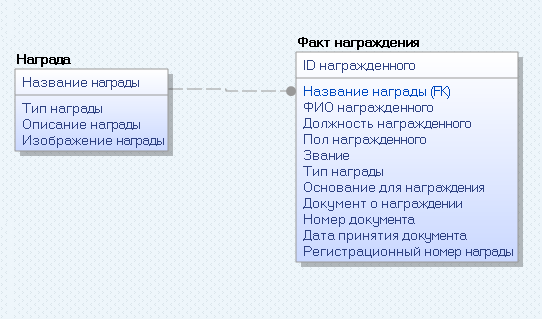
\includegraphics[width=130mm]{pic/er_naive.png}
  \caption{Исходная ER-модель \\ проектируемой базы данных}
  \label{fig:er_naive}
\end{figure}

Нетрудно заметить, что данная модель обладает недостатками:
\begin{itemize}
\item
  \textit{дублирование данных}: данные о каждом документе,
  подтверждающем факт награждения
  (<<документ о награждении>>, <<номер документа>>, 
  <<дата принятия документа>>) многократно дублируются и хранятся столько раз,
  сколько имеется объектов <<факт награждения>>;
\item
  \textit{аномалии удаления}: при удалении объекта <<награда>> удаляются все сведения
  о лицах, которые были ею награждены;
\item
  \textit{аномалии обновления}: при изменении значений <<тип награды>> в объекте
  <<награда>> появляется необходимость изменять все соответствующие вхождения этого свойства в
  объекты <<факт награждения>>.
\end{itemize}

\paragraph{}
С целью уменьшения дублирования данных и исключения аномалий введем
следующие объекты предметной области:

\begin{itemize}
\item <<награжденный>> --- хранит информацию о лице, предоставленным
  к государственной награде: ФИО, должность, пол, звание, место работы;
\item <<документ о награждении>> --- хранит информацию о документах,
  в которых перечислены списки лиц, предоставленных к награде: номер документа,
  название, дату принятия.
\end{itemize}

Объект <<награжденный>> может быть связан с несколькими
объектами <<факт награждения>> и каждый объект <<факт награждения>> 
соответствует единственному объекту <<награжденный>>.
Каждому объекту <<документ о награждении>> может соответствовать несколько
объектов <<факт награждения>> и каждому объекту <<факт награждения>> 
соовтетсвует единственный объект типа <<документ о награждении>>.

Кроме этого, проектируемый сервис должен поддерживать возможность ведения
учетных записи администраторов сервиса.
Cведения об учетных записях администраторов разумно также
расположить в базе данных. Для этого введем новый объект <<учетная запись>>,
который будет должен хранить следующие данные:
имя пользователя, пароль (в зашифрованном виде), адрес электронной почты.

\pagebreak
\paragraph{}
Окончательная ER-модель проектируемой базы данных с учетом
дополнительных объектов предметной области приведена
на рисунке~\ref{fig:er_final}.

\begin{figure}[h]
  \centering
  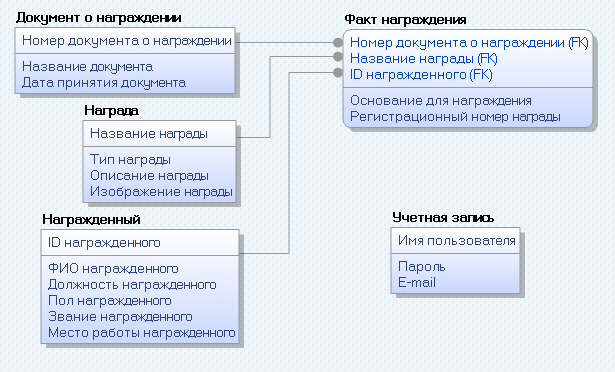
\includegraphics[width=150mm]{pic/er_final.png}
  \caption{Окончательная ER-модель \\ проектируемой базы данных}
  \label{fig:er_final}
\end{figure}

Нетрудно убедиться,
что хранение данных в соответствии с модифицированной моделью не имеет
недостатков, перечисленных ранее.

Таким образом, в ходе инфологического проектирования были описаны основные
сценарии использования базы данных, формат и содержания входных и выходных файлов
объекты предметной области и связи между ними, разработана ER-модель, лишенная
недостатков дублирования данных и аномалий.

\subsection{Даталогическое проектирование}
\label{ssub:db_data_stage}

\paragraph{}
Приведем несколько определений, которые потребуются для описания процесса
даталогического проектирования, взятых из авторитетного источника~\cite{date05}.

\textit{Модель данных} --- это абстрактное, самодостаточное,
логическое определение объектов, операторов и прочих элементов,
в совокупности составляющих абстрактную  машину доступа к данным,
с которой взаимодействует пользователь.

Реляционная модель данных состоит из трех частей:
\begin{itemize}
\item
  \textit{структурная часть} описывает, какие объекты рассматриваются
  реляционной моделью.
  Единственной структурой данных, используемой в реляционной модели,
  являются \textit{нормализованные отношения}.
\item
  \textit{целостная часть} описывает ограничения специального вида,
  которые должны выполняться для любых отношений в любых реляционных базах данных.
  Это \textit{целостность сущностей} и \textit{целостность внешних ключей}.
\item
  \textit{манипуляционная часть} описывает два эквивалентных способа
  манипулирования реляционными данными --- \textit{реляционную алгебру} и
  \textit{реляционное исчисление}.
\end{itemize}

\textit{Нормализацией отношений} базы данных называется процесс приведения каждого отношения
(таблицы) этой базы данных к определенной нормальной форме.
Нормализация каждого отношения выполняется поэтапно:
сначала отношение приводится к первой нормальной форме, затем --- ко второй, и~т.~д.
При переходе к каждой последующей нормальной форме устраняются недостатки
(\textit{аномалии}), присущие предыдущей нормальной форме.

Приведем формальные определения первых трех нормальных форм, 
взятые из источника~\cite{date05}. 

Переменная отношения находится в \textit{первой нормальной форме} тогда
и только тогда, когда в любом допустимом значении этой переменной отношения каждый
ее кортеж содержит только одно значение для каждого из атрибутов.

Переменная отношения находится во \textit{второй нормальной форме} тогда и только тогда,
когда она находится в первой нормальной форме и каждый неключевой атрибут
неприводимо зависит от ее первичного ключа.

Переменная отношения находится в \textit{третьей нормальной форме} тогда и только тогда,
когда она находится во второй нормальной форме и ни один неключевой атрибут не является
транзитивно зависимым от ее первичного ключа.

Следует отметить, что существуют также нормальные формы более высоких порядков,
но они реже используются в практических целях.  

\paragraph{}
Результатом даталогического проектирования является \textit{схема базы данных},
рассчитанная на конкретную СУБД, и удовлетворяющая следующим требованиям:
\begin{itemize}
  \item минимальная избыточность хранимых данных;
  \item минимальный физический объем данных;
  \item минимальное время доступа к данным;
  \item сокращение риска потери или искажения данных про внесении изменений в БД.
\end{itemize}

Для того, чтобы удовлетворить приведенные выше требования, достаточно проверить факт
нахождения отношений базы данных в определенной (как минимум, третьей) нормальной форме.
В том случае, когда отношение не отвечает требованиям определенной нормальной формы,
необходимо провести процедуру нормализации отношения.

\paragraph{}
На основании ER-модели, разработанной в подразделе~\ref{ssub:db_info_stage}, 
построим даталогическую модель базы данных.
Каждому объекту на рисунке~\ref{fig:er_final} соответствует отдельное отношение
проектируемой базы данных. 

Схема даталогической модели проектируемой базы данных, разработанная в среде проектирования CA ERWin, 
показана на рисунке~\ref{fig:er_physical}.

\begin{figure}[h]
  \centering
  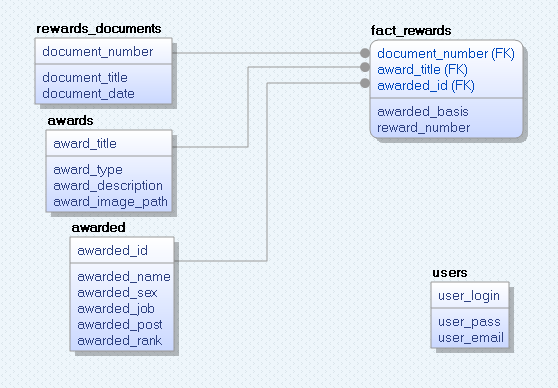
\includegraphics[width=150mm]{pic/er_physical.png}
  \caption{Даталогическая модель проектируемой базы данных}
  \label{fig:er_physical}
\end{figure}

\paragraph{}
Объекту <<документ о награждении>> соответствует отношение \textit{<<rewards\_documents>>},
схема которого приведена в таблице~\ref{tbl:rewards_documents_scheme}.

\begin{table}[h!]
  \caption{Схема отношения \textit{<<rewards\_documents>>}}
  \label{tbl:rewards_documents_scheme}
  \small{
    \centering
    \begin{tabular}{| p{0.3\textwidth} | p{0.25\textwidth} | p{0.2\textwidth} | p{0.14\textwidth} |}
      \hline
      Название атрибута \newline в модели &
      Название атрибута \newline в отношении &
      Тип хранимых \newline значений &
      Примечания \\ \hline

      Номер документа \newline о награждении &
      document\_number &
      INTEGER & Первичный ключ \\
      \hline

      Название документа &
      document\_title &
      VARCHAR(255) & \\
      \hline

      Дата принятия документа &
      document\_date &
      DATE & \\
      \hline

    \end{tabular}
  }
\end{table}

<<Номер документа о награждении>> принимает только целочисленные значения, следовательно, его можно хранить как 
целое число. <<Название документа>> может быть достаточно длинным и длина его может значительно колебаться
у различных записей. <<Дата принятия документа>> имеет стандартный тип DATE.

Покажем, что отношение \textit{<<rewards\_documents>>} находится в третьей нормальной форме:
\begin{itemize}
\item
все атрибуты отношения принимают простые значения
(условие первой нормальной формы);
\item
все неключевые атрибуты зависят от простого ключа
(условие пребывания отношения во второй нормальной форме);
\item
в отношении нет ни одной транзитивной функциональной зависимости от потенциального ключа
(условие пребывания отношения в третьей нормальной форме).
\end{itemize}

\paragraph{}
Объекту <<награда>> соответствует отношение \textit{<<awards>>},
схема которого приведена в таблице~\ref{tbl:awards_scheme}.

\begin{table}[h!]
  \caption{Схема отношения \textit{<<awards>>}}
  \label{tbl:awards_scheme}
  \small{
    \centering
    \begin{tabular}{| p{0.27\textwidth} | p{0.23\textwidth} | p{0.19\textwidth} | p{0.2\textwidth} |}
      \hline
      Название атрибута \newline в модели &
      Название атрибута \newline в отношении &
      Тип хранимых \newline значений &
      Примечания \\ \hline

      Название награды &
      award\_title &
      VARCHAR(255) &
      первичный ключ \\
      \hline

      Тип награды &
      award\_type &
      VARCHAR(20) & \\
      \hline

      Описание награды &
      award\_description &
      VARCHAR(255) & \\
      \hline

      Изображение награды &
      award\_image\_path &
      VARCHAR(255) & \\
      \hline
    \end{tabular}
  }
\end{table}

<<Название награды>> является уникальным, следовательно, его можно использовать
в качестве первичного ключа.
<<Тип награды>> может принимать достаточно короткие строковые значения
из заданного списка.
Длина <<описания награды>> может быть весьма значительной.
<<Изображение награды>> представляет собой системный путь к изображению награды
в файловой системе сервера.

Нетрудно убедиться, что отношение \textit{<<awards>>} находится 
в третьей нормальной форме.

\paragraph{}
Объекту <<награжденный>> соответствует отношение \textit{<<awarded>>},
схема которого приведена в таблице~\ref{tbl:awarded_scheme}.

\begin{table}[h!]


  \caption{Схема отношения \textit{<<awarded>>}}
  \label{tbl:awarded_scheme}
  \small{
    \centering
    \begin{tabular}{| p{0.23\textwidth} | p{0.25\textwidth} | p{0.2\textwidth} | p{0.23\textwidth} |}
      \hline
      Название атрибута \newline в модели &
      Название атрибута \newline в отношении &
      Тип хранимых \newline значений &
      Примечания \\ \hline

      ID награжденного &
      awarded\_id &
      INTEGER &
      первичный ключ \\
      \hline

      ФИО награжденного &
      awarded\_name &
      VARCHAR(255) & \\
      \hline

      Пол награжденного &
      awarded\_sex &
      CHAR &
      принимает значения 'm' или 'w' \\
      \hline

      Место работы \newline награжденного &
      awarded\_job &
      VARCHAR(255) & \\
      \hline

      Должность \newline награжденного &
      awarded\_post &
      VARCHAR(255) & \\
      \hline

      Звание \newline награжденного &
      awarded\_rank &
      VARCHAR(255) & \\
      \hline

    \end{tabular}
  }
\end{table}

<<ID награжденного>> является первичным ключом и имеет целочисленный тип.
<<ФИО награжденного>> является строкой и может иметь значительную длину.
<<Пол награжденного>> представляет собой символ, определяющий пол.
<<Должность награжденного>> является строкой и может иметь значительную длину.
<<Звание награжденного>> и <<место работы награжденного>> представляют собой строки переменной длины.

Нетрудно убедиться, что отношение \textit{<<awards>>} находится в третьей
нормальной форме.

\paragraph{}
Объекту <<факт награждения>> соответствует отношение \textit{<<fact\_rewards>>},
схема которого приведена в таблице~\ref{tbl:fact_rewards_scheme}.

\begin{table}[h!]
  \caption{Схема отношения \textit{<<fact\_rewards>>}}
  \label{tbl:fact_rewards_scheme}
  \small{
    \centering
    \begin{tabular}{| p{0.25\textwidth} | p{0.23\textwidth} | p{0.18\textwidth} | p{0.24\textwidth} |}
      \hline
      Название атрибута \newline в модели &
      Название атрибута \newline в отношении &
      Тип хранимых \newline значений &
      Примечания \\ \hline

      Номер документа \newline о награждении &
      document\_number &
      INTEGER &
      входит в первичный ключ \\
      \hline

      Название награды &
      award\_title &
      VARCHAR(255) &
      входит в первичный ключ \\
      \hline

      ID награжденного &
      awarded\_id &
      INTEGER &
      входит в первичный ключ \\
      \hline

      Основание \newline для награждения &
      awarded\_basis &
      VARCHAR(255) & \\
      \hline

      Регистрационный \newline номер награды &
      reward\_number &
      VARCHAR(20) & \\
      \hline

    \end{tabular}
  }
\end{table}

Атрибуты <<номер документа о награждении>>, <<название награды>>,
<<ID награжденного>> являются внешними ключами и входят в составной 
первичный ключ.
<<Основание для награждения>> является строкой переменной длины.
<<Регистрационный номер награды>> имеет строковый тип и принимает значения вида
<<1/13962>>, корректность которых проверяется регулярным выражением.

Покажем, что отношение \textit{<<fact\_rewards>>} находится в третьей нормальной форме:
\begin{itemize}
\item
  все атрибуты отношения принимают простые значения
  (требование первой нормальной формы);
\item
  все неключевые атрибуты зависят от простого ключа
  (требование второй нормальной формы); 
\item
  в отношении нет ни одной транзитивной функциональной зависимости
  от потенциального ключа (требование третьей нормальной формы).
\end{itemize}

\paragraph{}
Объекту <<учетная запись>> соответствует отношение \textit{<<users>>},
схема которого приведена в таблице~\ref{tbl:users_scheme}.

\begin{table}[h!]
  \caption{Схема отношения \textit{<<users>>}}
  \label{tbl:users_scheme}
  \small{
    \centering
    \begin{tabular}{| p{0.25\textwidth} | p{0.23\textwidth} | p{0.18\textwidth} | p{0.24\textwidth} |}
      \hline
      Название атрибута \newline в модели &
      Название атрибута \newline в отношении &
      Тип хранимых \newline значений &
      Примечания \\ \hline

      Имя пользователя &
      user\_login &
      VARCHAR(255) &
      Первичный ключ \\
      \hline

      Пароль &
      user\_pass &
      VARCHAR(255) & \\
      \hline

      E-mail &
      user\_email &
      VARCHAR(255) & \\
      \hline
    \end{tabular}
  }
\end{table}

Значения атрибута <<имя пользователя>> является уникальным, 
поэтому этот атрибут можно использовать в качестве первичного ключа.
Значения атрибута <<пароль>> представляет собой результат применения определенной хэш-функции
к строке пароля, вводимого пользователем.
Атрибут <<email>> имеет строковый тип переменной длины.

Нетрудно убедиться, что отношение \textit{<<users>>} находится в третьей
нормальной форме.

\paragraph{}
Таким образом, в ходе даталогического проектирования на основании ER-модели была разработана схема 
отношений базы данных.
Исходя из того, что все отношения проектируемой базы данных находятся в третьей нормальной форме,
можно утверждать, что вся база данных находится в третьей нормальной форме.


\subsection{Физическое проектирование}
\label{ssub:db_physical_stage}

На этапе физического проектирования производится перенос разработанной даталогической модели
на выбранное аппаратное и программное обеспечение.
Таким образом, результат данного этапа проектирования зависит от конкретной целевой платформы.
В нашем случае (смотри подраздел~\ref{ssec:choice_db}) целевой платформой является
реляционная СУБД MySQL 5.5.

Команды языка SQL, использованный для создания конфигупации таблиц,
соответствующей разработанной даталогической модели, 
приведены в приложении А.
